\section{Controlador local}
Para a intercomunicação entre os módulos e a nuvem, há a presença do servidor local, Morpheus, responsável por introduzir mais uma camada de segurança na troca de mensagens. Para isso, foi desenvolvida uma plataforma, com a utilização de sistemas de mensageria, e definido um protocolo de comunicação entre os serviços de nuvem e os módulos. Assim, quando um usuário realiza determinada operação por meio do cliente web, uma mensagem é enviada, interpretada pelo servidor local e, em seguida, encaminhada para o destino por meio do protocolo \wmqtt{} com o broker Mosquitto. O Morpheus é visto em detalhe na Seção \ref{chap:morpheus}.

\subsection{Raspberry Pi}
O Raspberry Pi é um computador integrado em um único chip, do tamanho de um cartão de crédito. Foi desenvolvido com o objetivo de promover o ensino de computação básica, e possui funcionalidades tais como um Computador Pessoal (PC): navegação na Internet, reprodução de video, processamento de texto, dentre outros. No projeto, será utilizado como servidor local (gerenciador de módulos local da casa), exatamente pelas funcionalidades compatíveis com a de um computador desktop.

A versão 3 possui uma CPU 1.2 Ghz 64-bit quad-core ARMv8, conexão 802.11n Wireless LAN, Bluetooth 4.1, suporte a Bluetooth Low Energy (BLE), 1GB RAM, 4 portas USB, 40 pinos GPIO, porta HDMI, porta Ethernet, interface para câmera, display e cartão SD. Para projetos que necessitem de baixo consumo energético, os modelos mais indicados são Pi Zero ou A+ \cite{raspPi}.

\begin{figure}[H]
	\centering
	\caption{Raspberry Pi 3 Modelo B}
  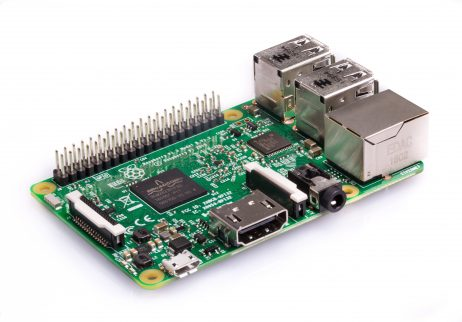
\includegraphics[width=0.5\textwidth]{Raspberry-Pi-3}
	\caption*{Fonte: \cite{raspPi}}
\label{fig:Raspberry-Pi-3}
\end{figure}
